%% Copyright 2015-2017 Angelos Drossos
%
% This work may be distributed and/or modified under the
% conditions of the LaTeX Project Public License, either version 1.3
% of this license or (at your option) any later version.

%% Presentation example
%
% LaTeX compiler support:
%  - PDFLaTeX
%  - LuaLaTeX
%

\RequirePackage{ifluatex}

% ---{{{ LuaLaTeX hotfix when ``pgfsys-luatex.def'' not found
% TexLive 2016 and MiKTeX
% (This hotfix must be defined before the beamer document class command.)
\ifluatex
\RequirePackage{luatex85}
\def\pgfsysdriver{pgfsys-pdftex.def}
\fi
% ---}}}

\documentclass[]{beamer}
\usepackage[%
	%english, % load babel with language english
	ngerman,  % load babel with language ngerman
	]{babel}
% one can change the font here
\ifluatex % --- packages needed when lualatex is used
\usepackage[%
	%math,    % load math packages
	]{fontspec}
\defaultfontfeatures{%
	Ligatures=TeX
	}
\setmainfont{Linux Libertine O}     % main font
\setsansfont{Linux Biolinum O}      % sans font (for sections)
\setmonofont{Linux LibertineMono O} % mono font (for listings)
\usepackage[%
	protrusion=true, %
	expansion,       %
	]{microtype}
\else % --- packages needed when pdflatex is used
\usepackage[T1]{fontenc}
\usepackage[utf8]{inputenc}
\usepackage[mono=true]{libertine} % main/sans/mono font (Libertine, Biolinum, LibertineMono)
\usepackage[%
	protrusion=true, %
	expansion,       %
	]{microtype}
\fi % --- end of lualatex/pdflatex specified packages

% This theme already initializes a HTWDD logo.
%   If you want to use another logo or want to clear the logo, define it with the logo command,
%   e.g.:
%   \logo{ABC}
%   \logo{}
%\logo{\includegraphics[height=0.8cm]{mylogo.pdf}}

% We want to use the HTWDD beamer theme.
%   In the HTWDD theme, the logo is rendered only once,
%   thus a customized logo must be set with the \logo command
%   before the \usetheme command is used.
\usetheme{HTWDD}

% set here your title, titlegraphic, date, author, institute
\title[My Presentation]{My HTWDD presentation}
%\subtitle{This is an example presentation} % -- note that a subtitle is not supported by HTWDD beamer theme until now
\titlegraphic{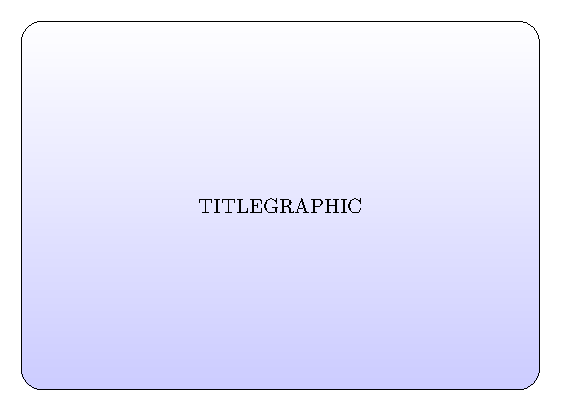
\includegraphics[height=4cm]{titlegraphic/titlegraphic-example.pdf}} % your titlegraphic as pdf or similar
\author[A.~Drossos]{Angelos~Drossos}
\institute[HTWDD]{University of Applied Sciences Dresden}
\date{\today} % if no date is specified, today is used
\subject{HTWDD Beamer Theme} % presentation subject
\keywords{HTWDD, LaTeX, Beamer, Theme, TikZ} % keywords describing the presentation

\begin{document}

%
% title page
%

\frame[plain]{\titlepage}
%\frame{\titlepage}

%
% outline (without subsections)
%
\section*{Outline}

\begin{frame}{Outline}
	\tableofcontents[hideallsubsections]
\end{frame}

%
% section: introduction
%
\section{Introduction}

\begin{frame}{\secname{}}
	\tableofcontents[currentsection,currentsubsection,hideothersubsections]
\end{frame}

\begin{frame}{I am a frame title -- and that is good so}
Hallo, I am a text inside a frame.

\vfill

\begin{itemize}
\item and I am a text inside an itemize environment
\item and a second text
\item and more\ldots
\end{itemize}
\end{frame}


\begin{frame}{I am a frame title -- and that is good so}{And I am a subtitle.. bah!}
Hallo, I am a text inside a frame.

\vfill

\begin{itemize}
\item and I am a text inside an itemize environment
\item and a second text
\item and more\ldots
\end{itemize}
\end{frame}


%
% section: ...
%
\section{Bla Bli Blubb Blocks}

\begin{frame}{\secname{}}
	\tableofcontents[currentsection,currentsubsection,hideothersubsections]
\end{frame}

\subsection{Blocks without headers}

\begin{frame}{Blocks}{without headers}
\begin{block}{}
\begin{itemize}
\item and I am a text inside an itemize environment
\item and a second text
\end{itemize}
\end{block}

\vfill

\begin{exampleblock}{}
\begin{itemize}
\item and I am a text inside an itemize environment
\item and a second text
\end{itemize}
\end{exampleblock}

\vfill

\begin{alertblock}{}
\begin{itemize}
\item and I am a text inside an itemize environment
\item and a second text
\end{itemize}
\end{alertblock}
\end{frame}


\subsection{Blocks with headers}

\begin{frame}{Blocks}{with headers}
\begin{block}{a fact}
\begin{itemize}
\item and I am a text inside an itemize environment
\item and a second text
\end{itemize}
\end{block}

\vfill

\begin{exampleblock}{an example}
\begin{itemize}
\item and I am a text inside an itemize environment
\item and a second text
\end{itemize}
\end{exampleblock}

\vfill

\begin{alertblock}{an alert!!}
\begin{itemize}
\item and I am a text inside an itemize environment
\item and a second text
\end{itemize}
\end{alertblock}
\end{frame}


\begin{frame}{Blocks}{overfull frame}
\begin{block}{a fact}
\begin{itemize}
\item and I am a text inside an itemize environment
\item and a second text
\end{itemize}
\end{block}

\vfill

\begin{exampleblock}{an example}
\begin{itemize}
\item and I am a text inside an itemize environment
\item and a second text
\item and more\ldots
\end{itemize}
\end{exampleblock}

\vfill

\begin{alertblock}{an alert!!}
\begin{itemize}
\item my text is not fully visible
\item Can you see this text?
\item Why you see this text?
\end{itemize}
\end{alertblock}
\end{frame}



%
% section: ...
%
\section{Overlays}

\begin{frame}{\secname{}}
	\tableofcontents[currentsection,currentsubsection,hideothersubsections]
\end{frame}

\begin{frame}{I am a frame title -- and that is good so}{And I am a subtitle.. bah!}
Hallo, I am a text inside a frame.

\vfill

\begin{block}{Overlays}
\begin{itemize}
\item<+-> and I am a text inside an itemize environment
\item<+-> and a second text
\item<+-> and more\ldots
\end{itemize}
\end{block}
\end{frame}


%
% APPENDIX (if needed)
%
\appendix

% Variant A: empty frame with text 'appendix'
\begin{frame}[plain]{\appendixname{} (Variant A)}
	\centering
	\usebeamerfont{title}%
	\usebeamercolor[fg]{structure}%
	\appendixname
\end{frame}

% Variant B: table of content of appendix
\begin{frame}{\appendixname{} (Variant B)}
	\tableofcontents[hideallsubsections]
\end{frame}

%
% appendix section: ...
%
\section{A1}

\begin{frame}{A CDEF}
	A text inside an appendix frame.
\end{frame}

%
% appendix section: ...
%
\section{B1}

\begin{frame}{B GHIJK}
	Another text inside an appendix frame.
\end{frame}


\end{document}
